\documentclass[10pt,twoside]{article}
\usepackage[utf8]{inputenc}
\usepackage{amsmath}
\usepackage{amsfonts}
\usepackage{amssymb}
\usepackage[spanish,es-noshorthands]{babel}
\usepackage[T1]{fontenc}
\usepackage{lmodern}
\usepackage{graphicx,hyperref}
\usepackage{tikz,pgf}
\usepackage{multicol}
\usepackage{subfig}
\usepackage[papersize={6.5in,8.5in},width=5.5in,height=7in]{geometry}
\usepackage{fancyhdr}
\pagestyle{fancy}
\fancyhead[LE]{
\includegraphics[height=12pt]{Images/logo-colegio.png} Aritmética $6^{\circ}$}
\fancyhead[RE]{}
\fancyhead[RO]{\textit{Germ\'an Avenda\~no Ram\'irez, Lic. U.D., M.Sc. U.N.}}
\fancyhead[LO]{}

\author{Germ\'an Avenda\~no Ram\'irez, Lic. U.D., M.Sc. U.N.}
\title{\begin{minipage}{.2\textwidth}

\includegraphics[height=1.75cm]{Images/logo-colegio.png}
\end{minipage}
\begin{minipage}{.55\textwidth}
\begin{center}
Taller 10, Operaciones en $\mathbb{N}$ \\
Aritm\'{e}tica $6^{\circ}$
\end{center}
\end{minipage}\hfill
\begin{minipage}{.2\textwidth}

\includegraphics[height=1.75cm]{Images/logo-sed.png} 
\end{minipage}}
\date{}
\begin{document}
\maketitle
Nombre: \hrulefill Curso: \underline{\hspace*{44pt}} Fecha: \underline{\hspace*{2.5cm}}
\section*{Continuaci\'{o}n taller anterior}
Lee la información y realiza lo que se indica en cada caso.\\

\begin{minipage}{.45\textwidth}
\begin{center}
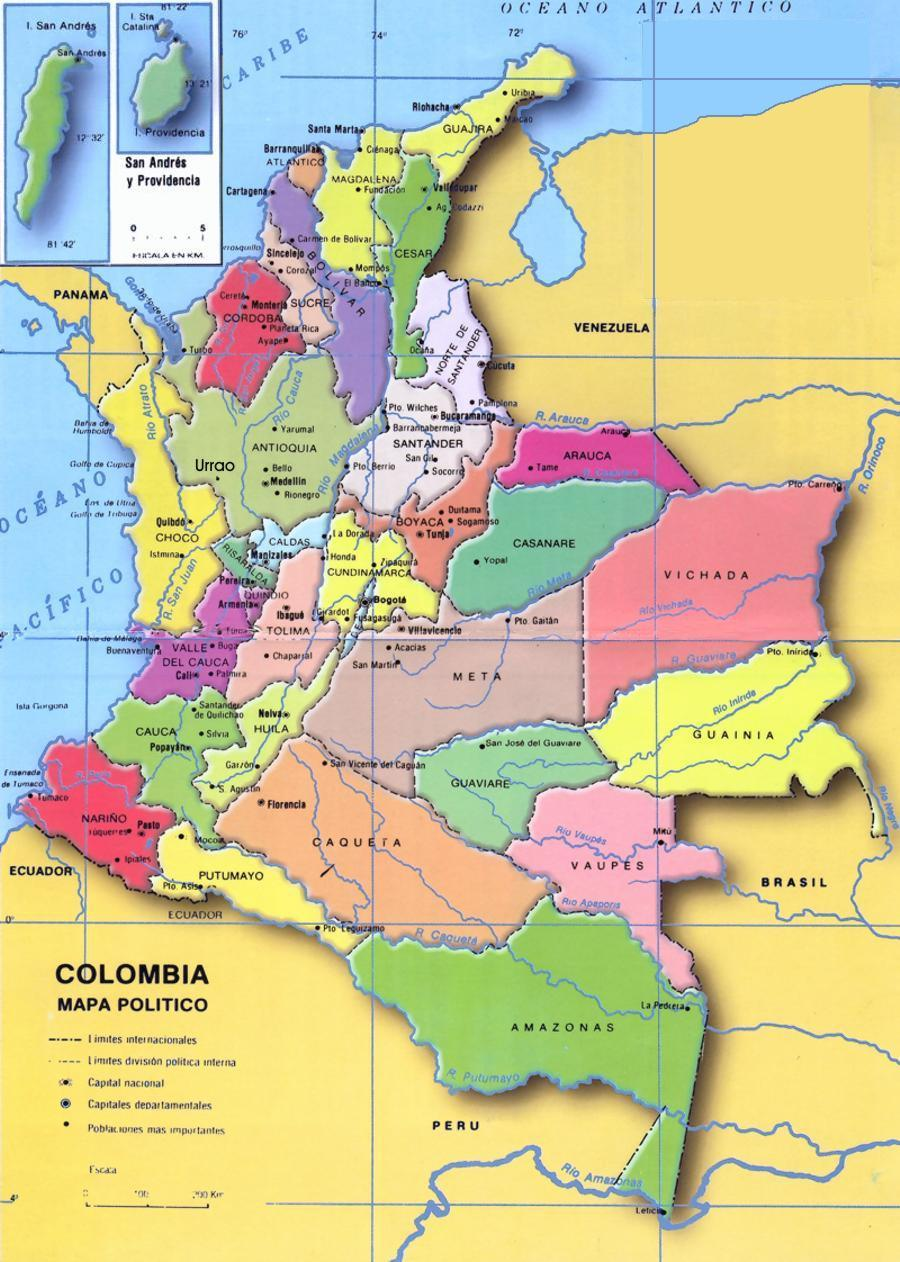
\includegraphics[scale=.7]{Images/mapa_colombia.jpg} 
\end{center}
\end{minipage}\hfill
\begin{minipage}{.5\textwidth}
La superficie terrestre de nuestro país está conformada por una parte continental y otra parte insular. La superficie de la parte continental es de 1'141\,748 km$^{2}$. 

Las aguas territoriales son las franjas de mar. Colombia tiene un área marítima de 930\,893 km$^{2}$.

El espacio aéreo está compuesto por una capa atmosférica de 2'083\,406 km$^{2}$. 

El subsuelo es la parte ubicada debajo de la superficie
\end{minipage}
\begin{itemize}
\item Escribe una pregunta que utilice los datos del espacio
colombiano y se resuelva con una adición.
\item Escribe una pregunta en donde se requiera una
sustracción.
\item Resuelve las preguntas que escribiste en los literales
anteriores.
\item Enuncia un problema que pueda plantearse a partir de la
información proporcionada.
\end{itemize}
Don Ramón quiere comprar una bicicleta y el vendedor le
informa que tiene las siguientes opciones de pago:
\begin{itemize}
\item Si paga de contado, le cuesta \$ 1'850\,000.
\item Puede pagar con cuatro cheques de \$ 470\,180: uno al
día y los otros a 30, 60 y 90 días.
\item Puede pagar la mitad y dos cheques posfechados de \$
580\,000 cada uno.
\item Puede pagar en doce cuotas de \$ 190\,000 cada una.
\end{itemize}
¿Cuál es la mejor opción para don Ramón? Explica tu
respuesta.
\section*{Actividad 2}
\begin{enumerate}
\item ¿Por qué son necesarios los números? ¿Para qué sirven? Pon ejemplos, sacados del periódico en los que se utilicen los números naturales para contar, ordenar e identificar.
\item Expresa en forma ordinal (se refiere a orden, como primero, segundo, tercero, etc) y escribe el nombre de los números siguientes: 20, 73, 85, 100.
\item Comprueba que el cero es el elemento neutro\footnote{Elemento neutro es el que no altera al número con el que se opera} de la suma y el uno el de la multiplicación. Explica por qué
\item Escribe las dos restas asociadas a cada suma:
\begin{enumerate}
\begin{multicols}{2}
\item $45+56=101$
\item $38+72=110$
\item $95+125=220$
\item $275+125=400$
\end{multicols}
\end{enumerate}
\item Escribe la suma y la resta asociadas a las siguientes restas:
\begin{enumerate}
\begin{multicols}{2}
\item $75-23=52$
\item $97-48=49$
\item $126-38=88$
\item $125-75=400$
\end{multicols}
\end{enumerate}
\item Realiza las siguientes operaciones combinadas:
\begin{enumerate}
\begin{multicols}{2}
\item $645-62\cdot 9+640\div 4+60=$
\item $600-25\cdot 6+512\div 8-89=$
\item $250\cdot 2\div 4+36-60\div 2=$
\item $(540-312)\cdot 15\div (75-4\cdot 15)=$
\end{multicols}
\end{enumerate}
\end{enumerate}
\end{document}
